%%%%%%%%%%%%%%%%%%%%%%%%%%%%%%%%%%%%%%%%%%%%%%%%
\section{Basic structure}


%%%%%%%%%%%%%%%%%%%%%%%%%%%%%%%%%%%%%%%%%%%%%%%%%%%%%%%
\begin{frame}

\frametitle{Basic format}

Like Make, a Snakemake file consists of a series of rules
\begin{itemize}
  \item While the format is different from Make, each rule has:
    \begin{itemize}
      \item A name
      \item Series of directives:
      \begin{enumerate}
        \item Input(s)
        \item Output(s)
        \item Command(s) to run to convert the inputs to the outputs
        \item ...
      \end{enumerate}
    \end{itemize}
  \item Rules can be chained together and/or create branches.
  \item A rule is applied if the date/time of the input(s) is newer than the output(s).
\end{itemize}

\end{frame}


%%%%%%%%%%%%%%%%%%%%%%%%%%%%%%%%%%%%%%%%%%%%%%%%%%%%%%%
\begin{frame}

\frametitle{Snakemake program}

The program is simply {\texttt{snakemake}}.
\vs

If the program is not installed on the machine you are using, then see the documentation on how to install it.
\vs

If you administer your own Linux machine, then you can install it with just {\texttt{sudo apt-get install snakemake}}.
\vs

Ubuntu 26.04 LTS will install version 7.32.4.  The latest version appears to be 9.27.1.

\end{frame}


%%%%%%%%%%%%%%%%%%%%%%%%%%%%%%%%%%%%%%%%%%%%%%%%%%%%%%%
\begin{frame}

\frametitle{Filename}

Like {\texttt{Make}}, when you run {\texttt{snakemake}}, it will search for a file of rules.  This file should be one of the following:
\begin{itemize}
  \item {\texttt{Snakefile}},
  \item {\texttt{snakefile}},
  \item {\texttt{workflow/Snakefile}},
  \item {\texttt{workflow/snakefile}}
\end{itemize}
\vs

{\magenta{However}}, I tend to use the {\texttt{--snakefile}} option to specify my own filename:  {\texttt{Snakefile.smk}} (so that I can find my Snakemake files easily).
\vs

Like Python scripts which can be broken up into modules and ``imported'' in, the rules in a Snakemake file can be separated into multiple files and ``included'' in.

\end{frame}


%%%%%%%%%%%%%%%%%%%%%%%%%%%%%%%%%%%%%%%%%%%%%%%%%%%%%%%
\begin{frame}

\frametitle{Snakemake options}

See the manual for a list of options.  But besides {\texttt{--snakefile}}, I find these useful:
\begin{itemize}
  \item {\texttt{--cores}} -- number of cores to use; rules that are not dependent on each other can execute in parallel across multiple cores
  \item {\texttt{--dryrun}} -- perform a ``dry run'' (i.e., do not actually run)
  \item {\texttt{-p}} -- print shell commands
\end{itemize}

\end{frame}


%%%%%%%%%%%%%%%%%%%%%%%%%%%%%%%%%%%%%%%%%%%%%%%%%%%%%%%
\begin{frame}[fragile]

\frametitle{Sample Rule\footnote{V2}}

\begin{figure}
  \centering
  \begin{tabular}{lc}
DATA\_DIR = "../../data" & \only<7>{{\red{$\leftarrow$}}} \\
OUTPUT\_DIR = "Output" & \only<7>{{\red{$\leftarrow$}}} \\
\\
rule CountAlice: & \only<1>{{\red{$\leftarrow$}}} \\
  {\D\D}input:  DATA\_DIR + "/canterbury/alice29" & \only<2>{{\red{$\leftarrow$}}} \\
  {\D\D}output:  OUTPUT\_DIR + "/alice29.count" & \only<3>{{\red{$\leftarrow$}}} \\
  {\D\D}shell: & \only<4>{{\red{$\leftarrow$}}} \\
  {\D\D\D\D}""" & \only<5>{{\red{$\leftarrow$}}} \\
  {\D\D\D\D}cat \{input\} | head -n 1000 | wc -w -c >\{output\} & \only<6>{{\red{$\leftarrow$}}} \\
  {\D\D\D\D}""" & \only<5>{{\red{$\leftarrow$}}} \\
  \end{tabular}
\end{figure}

Note:  Variables are enclosed in curly braces.

\end{frame}


%%%%%%%%%%%%%%%%%%%%%%%%%%%%%%%%%%%%%%%%%%%%%%%%%%%%%%%
\begin{frame}

\frametitle{Sample Rule\footnote{V2}}

\begin{figure}
  \centering
  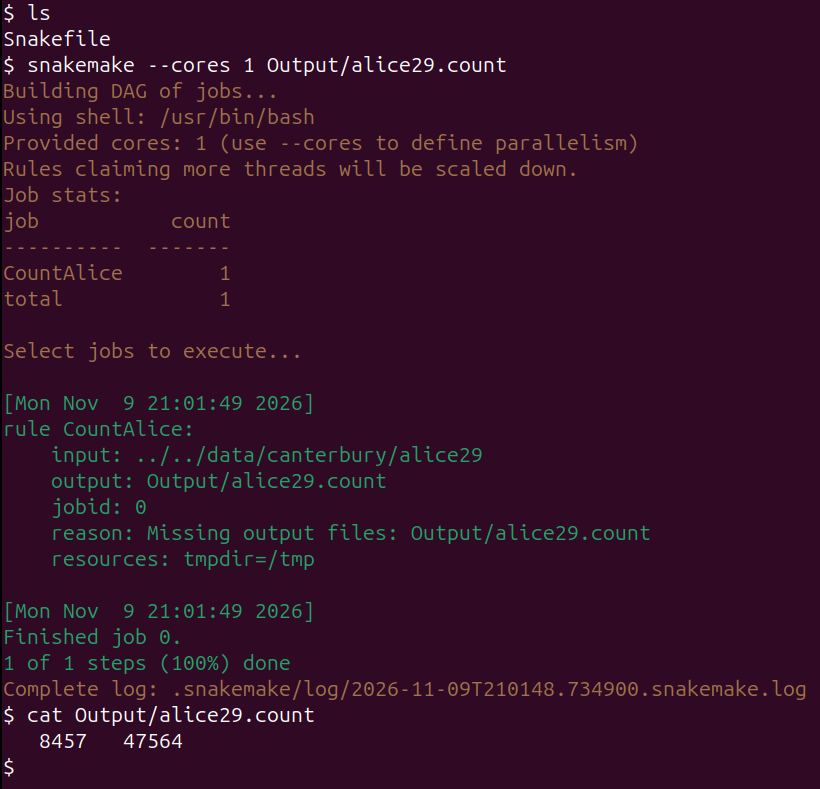
\includegraphics[height=7cm]{structure/example-v2}
\end{figure}

\end{frame}


%%%%%%%%%%%%%%%%%%%%%%%%%%%%%%%%%%%%%%%%%%%%%%%%%%%
\begin{frame}[fragile]

\frametitle{Example with two rules\footnote{V3}}

\begin{tiny}
\begin{lstlisting}[frame=single,language=bash]
DATA_DIR = "../../data"
OUTPUT_DIR = "Output"

rule TopAlice:
  input:  DATA_DIR + "/canterbury/alice29"
  output:  OUTPUT_DIR + "/01-top/alice29.head"
  shell:
    """
    head -n 1000 {input} >{output}
    """

rule CountAlice:
  input:  OUTPUT_DIR + "/01-top/alice29.head"
  output:  OUTPUT_DIR + "/02-count/alice29.count"
  shell:
    """
    wc -w -c {input} >{output}
    """
\end{lstlisting}
\end{tiny}

\end{frame}


%%%%%%%%%%%%%%%%%%%%%%%%%%%%%%%%%%%%%%%%%%%%%%%%%%%%%%%
\begin{frame}

\frametitle{Sample Rule\footnote{V3}}

\begin{figure}
  \centering
  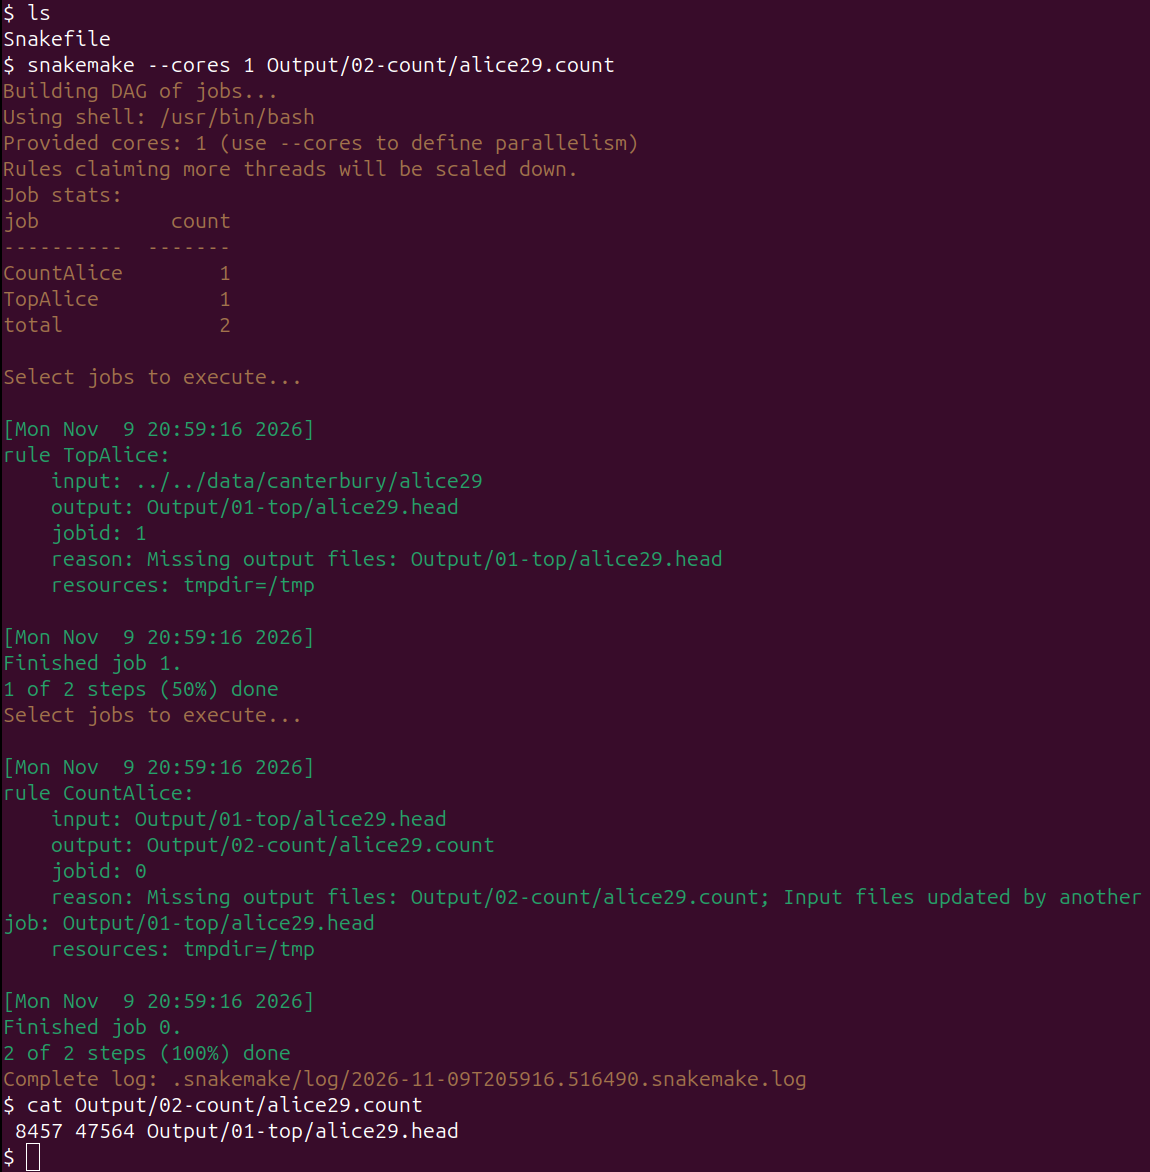
\includegraphics[height=7cm]{structure/example-v3}
\end{figure}

\end{frame}


%%%%%%%%%%%%%%%%%%%%%%%%%%%%%%%%%%%%%%%%%%%%%%%%%%%
\begin{frame}[fragile]

\frametitle{Generalising\footnote{V4}}

\begin{tiny}
\begin{lstlisting}[frame=single,language=bash]
##  Include important variables
include:  "global-vars.smk"

rule all:
  input:
    OUTPUT_DIR + "/02-count/alice29.count",
    OUTPUT_DIR + "/02-count/asyoulik.count",
    OUTPUT_DIR + "/02-count/lcet10.count",
    OUTPUT_DIR + "/02-count/plrabn12.count"

rule FileTop:
  input:  DATA_DIR + "/canterbury/{fn}"
  output:  OUTPUT_DIR + "/01-top/{fn}.head"
  shell:
    """
    head -n 1000 {input} >{output}
    """

rule Count:
  input:  OUTPUT_DIR + "/01-top/{fn}.head"
  output:  OUTPUT_DIR + "/02-count/{fn}.count"
  shell:
    """
    wc -w -c {input} >{output}
    """
\end{lstlisting}
\end{tiny}

\end{frame}


%%%%%%%%%%%%%%%%%%%%%%%%%%%%%%%%%%%%%%%%%%%%%%%%%%%
\begin{frame}[fragile]

\frametitle{Generalising\footnote{V4}}

In this example,
\begin{itemize}
  \item The path variables have been moved to a separate file called {\texttt{global-vars.smk}}.  That file has been included in.
  \item There is an {\magenta{all}} rule which has an input directive but no output directive.
    \begin{itemize}
      \item If it is first in the file, then it will be applied if you run Snakemake with no options.  (i.e., a ``default'' rule)
      \item Other rules can occur before it if they are included in (i.e., not before it in the same file).
    \end{itemize}
  \item Together, we can now process all four files by {\green{just}} adding them to the {\magenta{all}} rule.
\end{itemize}

\end{frame}



%%%%%%%%%%%%%%%%%%%%%%%%%%%%%%%%%%%%%%%%%%%%%%%%%%%%%%%
\begin{frame}

\frametitle{Generalising Results\footnote{V4}}

\begin{figure}
  \centering
  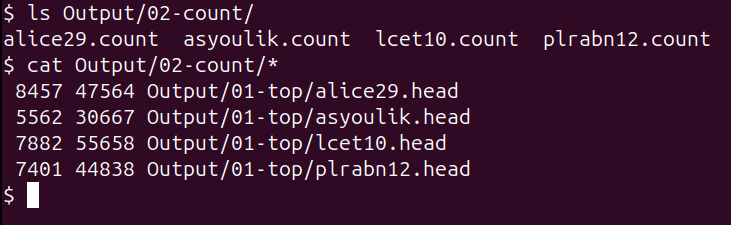
\includegraphics[width=9cm]{structure/example-v4}
\end{figure}

\end{frame}


%%%%%%%%%%%%%%%%%%%%%%%%%%%%%%%%%%%%%%%%%%%%%%%%%%%%%%%
\begin{frame}[fragile]

\frametitle{Visualisation\footnote{V4}}

Create a ``DAG'' (directed acyclic graph) for {\texttt{graphviz}} (not part of Snakemake):
\begin{tiny}
\begin{lstlisting}[frame=single,language=bash]
snakemake --cores 1 --dag | dot -Teps >dag.eps
\end{lstlisting}
\end{tiny}

\begin{figure}
  \centering
  {\fbox{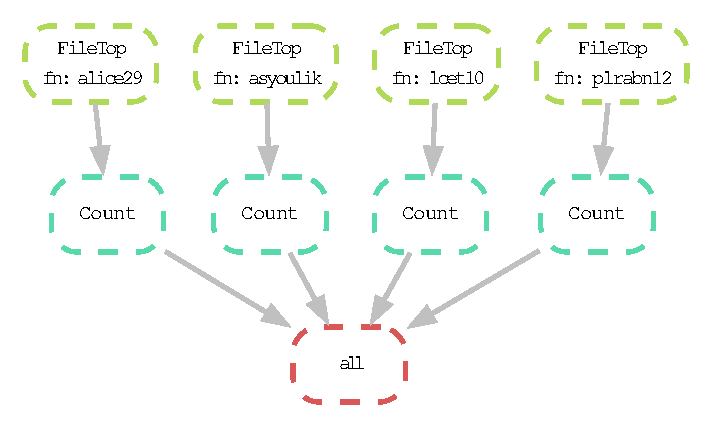
\includegraphics[width=7cm]{structure/dag-v4}}}
\end{figure}

\end{frame}


%%%%%%%%%%%%%%%%%%%%%%%%%%%%%%%%%%%%%%%%%%%%%%%%%%%%%%%
\begin{frame}[fragile]

\frametitle{Python instead of bash commands\footnote{V5}}

\begin{tiny}
\begin{lstlisting}[frame=single,language=python]
DATA_DIR = "../../data"
OUTPUT_DIR = "Output"

rule CountAlice:
  input:  DATA_DIR + "/canterbury/alice29"
  output:  OUTPUT_DIR + "/alice29.count"
  run:
    with open (output[0], "w") as outfp:
      with open (input[0]) as infp:
        num_words = 0
        num_chars = 0
        for line in infp:
          wordslist = line.split ()
          num_words = num_words + len (wordslist)
          num_chars += (sum (len (word) for word in wordslist))
      outfp.write (str (num_words))
      outfp.write ("\t")
      outfp.write (str (num_chars) + "\t" + output[0] + "\n")
\end{lstlisting}
\end{tiny}

\end{frame}


